% Speaker script for slides.tex.  Build: ./build.sh
% build_html.py converts this file into notes.html and into the notes panel of
% slides.html, so keep to the macros used here (\slidenote, \emph, \textbf,
% inline $...$ with \alpha \Psi \pi \Omega \kappa \times \approx \sim \to \ge \le \ne \rm,
% ^{} and _{}).
\documentclass[12pt,a4paper]{article}
\usepackage[T1]{fontenc}
\usepackage[utf8]{inputenc}
\usepackage{lmodern}
\usepackage[a4paper,margin=2.2cm]{geometry}
\usepackage{graphicx}
\usepackage{xcolor}
\usepackage{enumitem}
\usepackage[colorlinks=true,urlcolor=blue!55!black]{hyperref}
\definecolor{accent}{HTML}{1F5FA8}
\definecolor{muted}{HTML}{6B7280}
\setlength{\parindent}{0pt}
\setlength{\parskip}{6pt}
\linespread{1.12}

\newcommand{\slidenote}[3]{%
  \par\bigskip\noindent
  \begin{minipage}[t]{.3\textwidth}\vspace{0pt}
    \includegraphics[page=#1,width=\linewidth]{slides.pdf}
  \end{minipage}\hfill
  \begin{minipage}[t]{.66\textwidth}\vspace{0pt}
    {\large\bfseries\color{accent}#1.\ #2}\par
    {\small\color{muted}#3}
  \end{minipage}\par\smallskip}

\begin{document}

{\LARGE\bfseries Speaker script\par}
\smallskip
{\large Extremality shift of rotating black holes at finite Gauss--Bonnet coupling\par}
{\color{muted}Ten minutes, eight slides. About 1200 words at a calm pace; the ``Behind the numbers''
paragraph of slide 4 is background, not script. The times are targets;
the elapsed time is in brackets.\par}

\slidenote{1}{Title}{0:30 \quad [0:30]}

This is joint work by Cecilia Bejarano, David Blanco, Guillem Pérez-Nadal and
myself. Most of the code, the computations and the writing were done by two AI
agents, Claude Code and Codex, under our direction.

The talk has two halves: a physics result, and what it took to get it with agents.

\slidenote{2}{The question}{1:20 \quad [1:50]}

A rotating black hole cannot spin arbitrarily fast for a given mass. For Kerr, in
the box, $J \le M^2$. At the bound the two horizons merge and the temperature
vanishes: that is what \emph{extremal} means. The first law,
$dM = T\,dS + \Omega_H\,dJ$, compares neighbouring black holes.

In five dimensions with two equal angular momenta, the Myers--Perry solution, the
bound is $M \ge$ three halves $\pi^{1/3} J^{2/3}$, again saturated at zero
temperature. That is the orange star.

The bound belongs to the field equations. If we add the Gauss--Bonnet term, the
only quadratic curvature correction whose equations stay second order, with a
coupling $\alpha$, the bound moves.

At first order in $\alpha$ this is known: the extremal mass grows with slope
exactly $\pi$. That is the dashed line. Numerical solutions at finite coupling also
exist. But nobody had reported how the extremal mass changes once $\alpha$ is not
small, that is, its slope. That is the question mark, and that is what we measured.

\slidenote{3}{How it started: the first prompts}{1:25 \quad [3:15]}

The project began on September 4th, as the final project of this course. At the
top is the very first prompt, to Codex: write numerical codes for rotating black
holes in more than four dimensions, reproduce the literature, then look for new
solutions.

On the left, the roadmap the agent wrote on day two, as saved. Milestone 4,
reproducing Brihaye et al., was the ``minimum success''. Milestone 6, a ``new
exploration'' to be chosen after milestone 4, became the potential $\Psi$.
Milestone 8, zero temperature and the paper, was not planned at all.

On the right, the paper we reproduced. For $\alpha \ne 0$ it finds no simple Smarr
relation, and footnote 14 suggests extending the static Lovelock one of Kastor,
Ray and Traschen to spinning black holes. With $\alpha$ as a thermodynamic
variable, scaling gives it: $2M = 3TS + 6\Omega_H J + 2\alpha\Psi$, which our
solutions satisfy to about $10^{-7}$.

Later prompts were mostly short: ``continue with milestone 3'', ``go ahead''. The
human work was elsewhere: choosing the direction, reading, doubting, and making
each agent referee the other's work.

\slidenote{4}{Step 1: reproduce the published family}{1:30 \quad [4:45]}

Before measuring anything new, the solver has to reproduce what is known. These
are the four metric functions of the rotating solution at the coupling and spin of
Figure~1 of Brihaye, Kleihaus, Kunz and Radu, 2010. The lines are ours, the dots
are theirs.

We did not digitise the picture. The arXiv source contains the figure as vector
PostScript, so the agent read the exact vertices of each curve and calibrated the
axes from the file's own tick marks.

At the horizon we agree to two parts in ten thousand, less than half the plotting
resolution of their figure. In the interior the curves differ by up to about one
percent, which you see on the right. Is that our error? The same figure shows a
curve at almost zero coupling, where the exact solution is known in closed form,
and their plotted curve is also about one percent away from the exact formula.
So the gap is in the published plot, not in the solver, although we do not know
why.

One comparison did not close: the ergosurface radius, 1.1021 against the 1.104 in
the paper. We report it as an open discrepancy, not as an erratum.

\textbf{Behind the numbers} (background for you, not to read out). The figure is
at the paper's coupling $\alpha_{\rm ref} = 3$, which is $\alpha = 0.75$ in our
normalisation; $\alpha_{\rm ref} = 4\alpha$ is fixed by matching their entropy
formula to ours, not assumed. The horizon radius is $r_H = 1$ and the spin
$q = 0.33$. Each published curve gives 74 vertices, the dots.

\emph{$2\times10^{-4}$.} The largest difference at the horizon among the four
functions is $2.07\times10^{-4}$. Gnuplot writes integer coordinates, so their
figure cannot resolve less than one device unit, which in data units is
$5.2\times10^{-4}$; it is the shaded band on the right panel. We are at 0.4 of that
unit (the slide rounds this to ``a third''), that is, at the resolution of the
figure. The horizon values fix the parameters and the boundary conditions, so this
says we solved the same problem.

\emph{$\sim10^{-2}$.} The largest difference in the interior is $1.4\times10^{-2}$,
a smooth bump where the curves are steepest. That is some 27 device units, so it is
not rounding. The control is the curve the same figure draws at
$\alpha_{\rm ref} = 0.01$, where our solution is Myers--Perry to thirteen digits:
there the published curve sits $8.2\times10^{-3}$ from ours and $9.5\times10^{-3}$
from the closed form, which has no numerical error. A plotted curve that misses an
exact solution by that much cannot test ours more sharply than that. Where their
offset comes from is not known.

\emph{1.1021 vs 1.104.} This number is not read from the figure. The paper's text
(section 4.1.1) quotes the outer ergosurface radius, where $g_{tt} = 0$, at
$r_H = 1$ and $\Omega_H = 0.33$: 1.059, 1.08 and 1.104 for $\alpha_{\rm ref} = 0$, 1
and 2. We get 1.0593, 1.0791 and 1.1021. The first two agree within the rounding
of the printed digits. The third misses by $1.9\times10^{-3}$, almost four times
the largest rounding error of a number printed to three decimals. Matching it would need
$\alpha_{\rm ref} \approx 2.09$ instead of 2, and the normalisation is pinned
independently by the entropy. So it stays open. It tests the metric functions away
from the horizon and does not enter the charges, $\Psi$ or the extrapolation.

\slidenote{5}{Step 2: the measurement}{1:30 \quad [6:15]}

Now the new part. On the left are the four functions for all thirteen couplings,
$\alpha$ from zero to one half, at one spin. Each curve is a full nonlinear solve:
356 accepted solutions in total, with a spectral method and Newton iteration.

The key quantity is $\Psi$, the variable conjugate to $\alpha$ in the extended first
law, the equation at the top. $\Psi$ says how the mass changes when you change the
\emph{theory}, at fixed entropy and spin. At zero temperature the $T\,dS$ term
drops, and $\Psi$ becomes exactly the slope we are after. So a single solution
gives the slope; we never subtract nearby solutions.

The derivative in $\alpha$ is also exact: differentiating the discretised
equations gives one linear system, with the matrix Newton already built. That is
the implicit function theorem, so there is no step size to tune.

On the right is $\Psi$ against temperature for several couplings; the crosses are
the exact static solutions. The slope is where each curve reaches zero temperature,
on the left. We never build a zero-temperature solution: we get very cold and
extrapolate.

\slidenote{6}{Result}{1:30 \quad [7:45]}

Here is the result. On the left, the slope of the extremal mass against the scaled
coupling $y = \alpha/J^{2/3}$. At $y = 0$ we recover $\pi$, the green star, to about
one part in ten million. Then the slope falls fast, to a minimum near 1.07 at
$y \approx 0.18$, and rises again to 1.44 at the largest coupling we reached. The
open squares are an independent estimate from the mass curve, and they agree.

So, three statements. The slope is always positive: Gauss--Bonnet makes the spin
bound tighter. It is far from constant, so the linear formula fails beyond small
coupling. And it is not monotonic.

On the right is the extremal mass itself. It grows by 31 percent over the range,
and by the end the first-order line overshoots the shift by a factor 1.32. The
final rise is actually required: a known bound, $M > 3\pi\alpha/4$, would be
violated if the slope stayed low.

The caveat: every zero-temperature number is an extrapolation.

\slidenote{7}{How far can it be trusted?}{1:00 \quad [8:45]}

$\Psi$ from the linear solve has no closed form, so we tested it against things
that do not use it: the exact static solution, the published first-order result,
the Smarr relation, the on-shell Gauss--Bonnet action, the near-horizon entropy,
the field equations away from the grid, and a full rerun at lower resolution. The
worst deviations go from $10^{-11}$ to $10^{-4}$.

The referee rounds between the agents mattered too. One check that a referee asked
for \emph{failed} when it was run, and an exact bound exposed a real error in the
mass that three internal diagnostics had missed. What remains open is the extrapolation to zero temperature, equal spins
only, and a single branch of solutions.

\slidenote{8}{What it cost}{1:15 \quad [10:00]}

Finally, the cost. About 37 hours of active agent time, over 13 days in September,
and 79 human prompts. The agents processed 1.4 billion tokens, but 99 percent of
that is the context being re-read at every tool call. They \emph{wrote} about six
million tokens, some 24 megabytes of text: fourteen times the size of the final
product.

The expensive blocks, in orange, are building the rotating solver and the final
measurement with the paper. Reproducing all the known solutions took four hours.
The first genuinely new object, the rotating Gauss--Bonnet black hole, took five
times as many tokens; five solver strategies were thrown away before one worked.
None of this counts our own time, or the numerical runs in the background.

Our lesson: the cost was not in writing code. It was in verifying, failing,
catching mistakes and redoing, and that is also what makes the result defensible.
Everything, including the code, data, checks and prompts, is in the repository.
Thank you.

\newpage
\section*{If there are questions}

\begin{description}[leftmargin=0pt,style=nextline]
\item[Why is $J$ not like a charge, for the weak gravity conjecture?]
Angular momentum is not a gauge charge, so the WGC spectrum arguments do not
carry over. We use the Goon--Penco relation only as an identity of the first law,
and draw no WGC conclusion.
\item[Why not solve directly at $T=0$?]
Kleihaus, Kunz and Radu (2023) did build extremal solutions directly, in a
different gauge. Our solver works at a fixed horizon radius and angular velocity,
so we approach $T=0$. The spread over 21 fitting choices is reported as a
sensitivity, not an error bar.
\item[What exactly is new?]
$\Psi$ on rotating solutions at finite coupling; the slope at 13 couplings, with its
minimum and its rise; the extremal mass curve and how far it departs from first
order; and the reading of $\Psi$ as an on-shell Gauss--Bonnet action.
\item[Which parts did the humans do?]
We chose the problem and the reference papers, steered each milestone, asked for
critical reviews, made the agents referee each other, and questioned the results.
The agents wrote the code, ran it and drafted the text.
\end{description}

\section*{On crediting the AI}

AI tools cannot be authors, because they cannot take responsibility for the work.
That is the position of COPE and of Springer Nature, which publishes JHEP; arXiv
likewise holds the human authors responsible for everything submitted. Springer
Nature asks for a disclosure in the methods section or the acknowledgements, giving
each tool's name, version, maker and purpose. On the
title slide that is the line ``With AI assistance: Claude Code (Anthropic; Claude
Opus 5, Sonnet 5) and Codex (OpenAI; GPT-5)''. For the paper, a sentence such as:
``Code, numerical computations and a first draft were produced with Claude Code
(Anthropic) and Codex (OpenAI) under the authors' direction; the authors checked
the results and take full responsibility for the content.''

\end{document}
